\section{Data Collection and Graph Generation}

Every time a latency test, a test run to see the impact of delay on the prototype's
latency, has finished running it will contact the logger at /stat to get the 
data and write in a JSON file:
  
\begin{listing}[!ht]
  \begin{minted}{json}
[
  {
    "delay_time": "0.0",
    "latency": 0.04399871826171875
  },
  ...
]
  \end{minted}
  \caption{Latency data obtain from the logger}
\end{listing}

% The JSON file is written in the following 
% format: algorithm\_name\_\%Y-\%m-\%d\_\%H-\%M-\%S.json. For example a file name could be
% maekawa\_2023-06-07\_09-21-36.json where \textit{maekawa} is the name of the algorithm
% and the rest of the file name is the date and time that it was first written.

By using the value of \textit{delay\_time} as the horizontal x-axis and the \textit{latency}
as the vertical y-axis along with tool such as numpy and matplotlib we can generate the following 
graphs:

\begin{figure}[htbp]
  \centering
  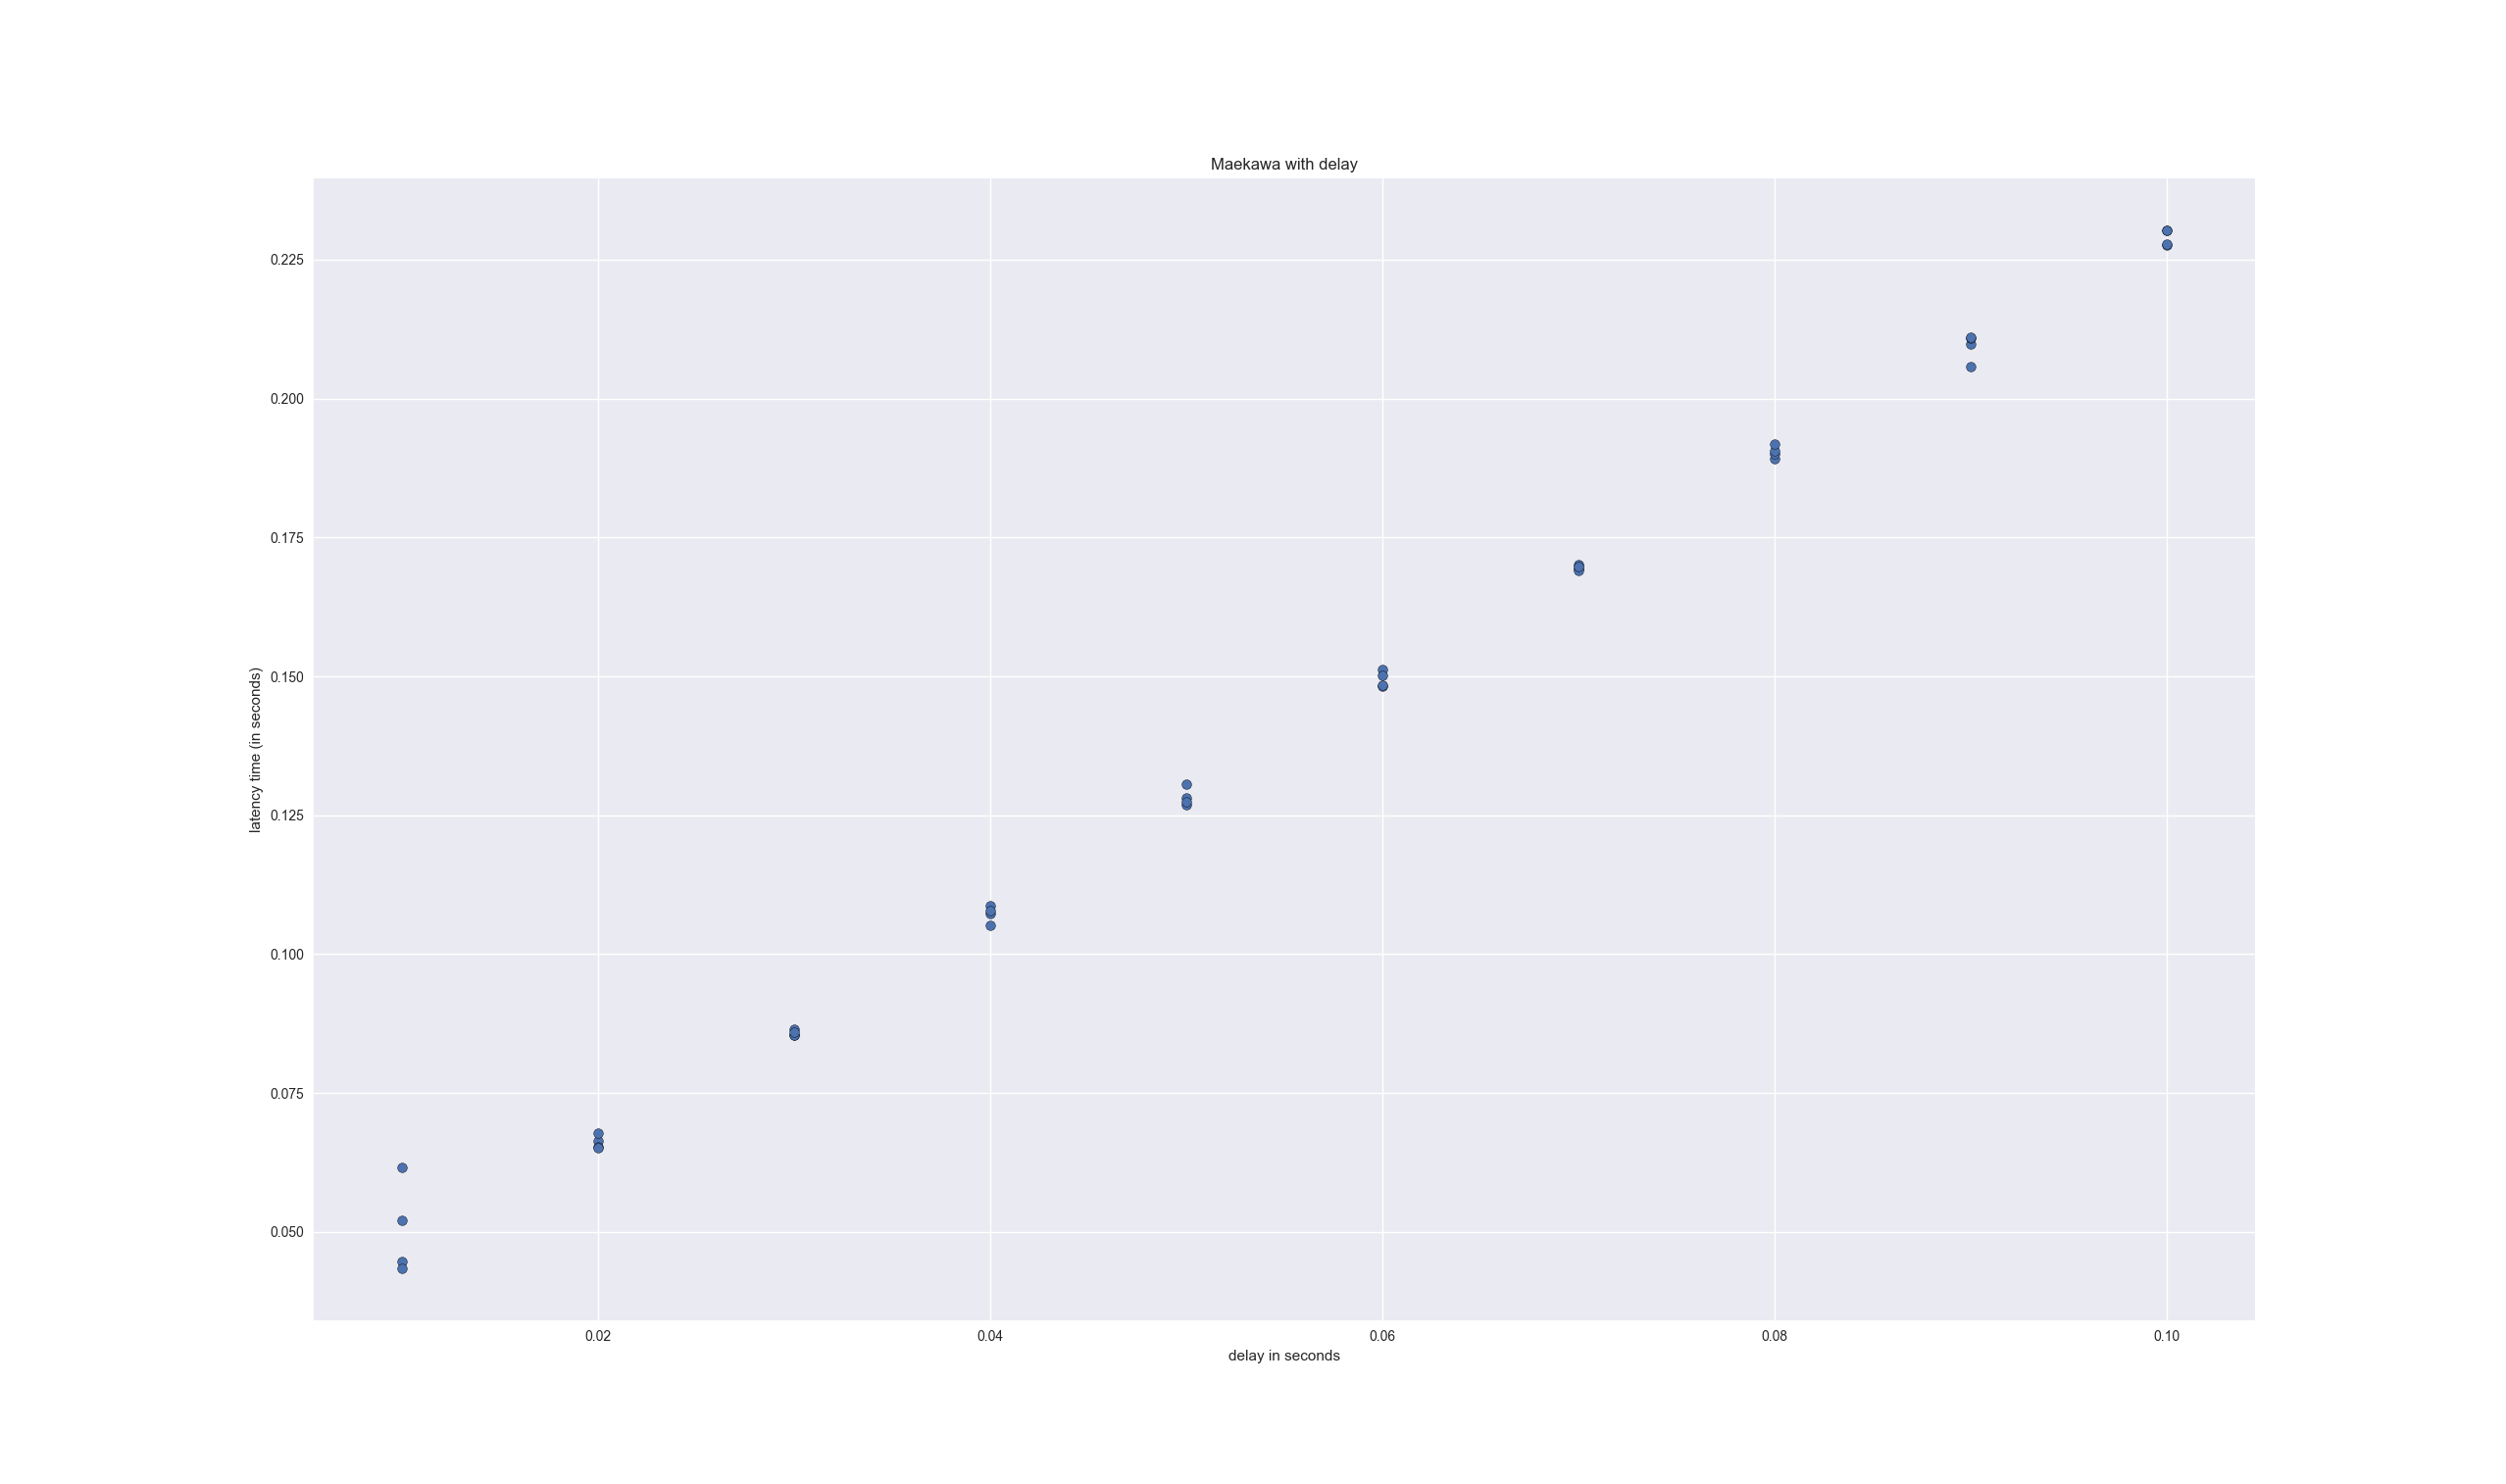
\includegraphics[width=\linewidth,height=\textheight,keepaspectratio]{maekawa_delay.png}
  \caption{Scatter plot between latency and delay in Maekawa algorithm}
\end{figure}

\begin{figure}[htbp]
  \centering
  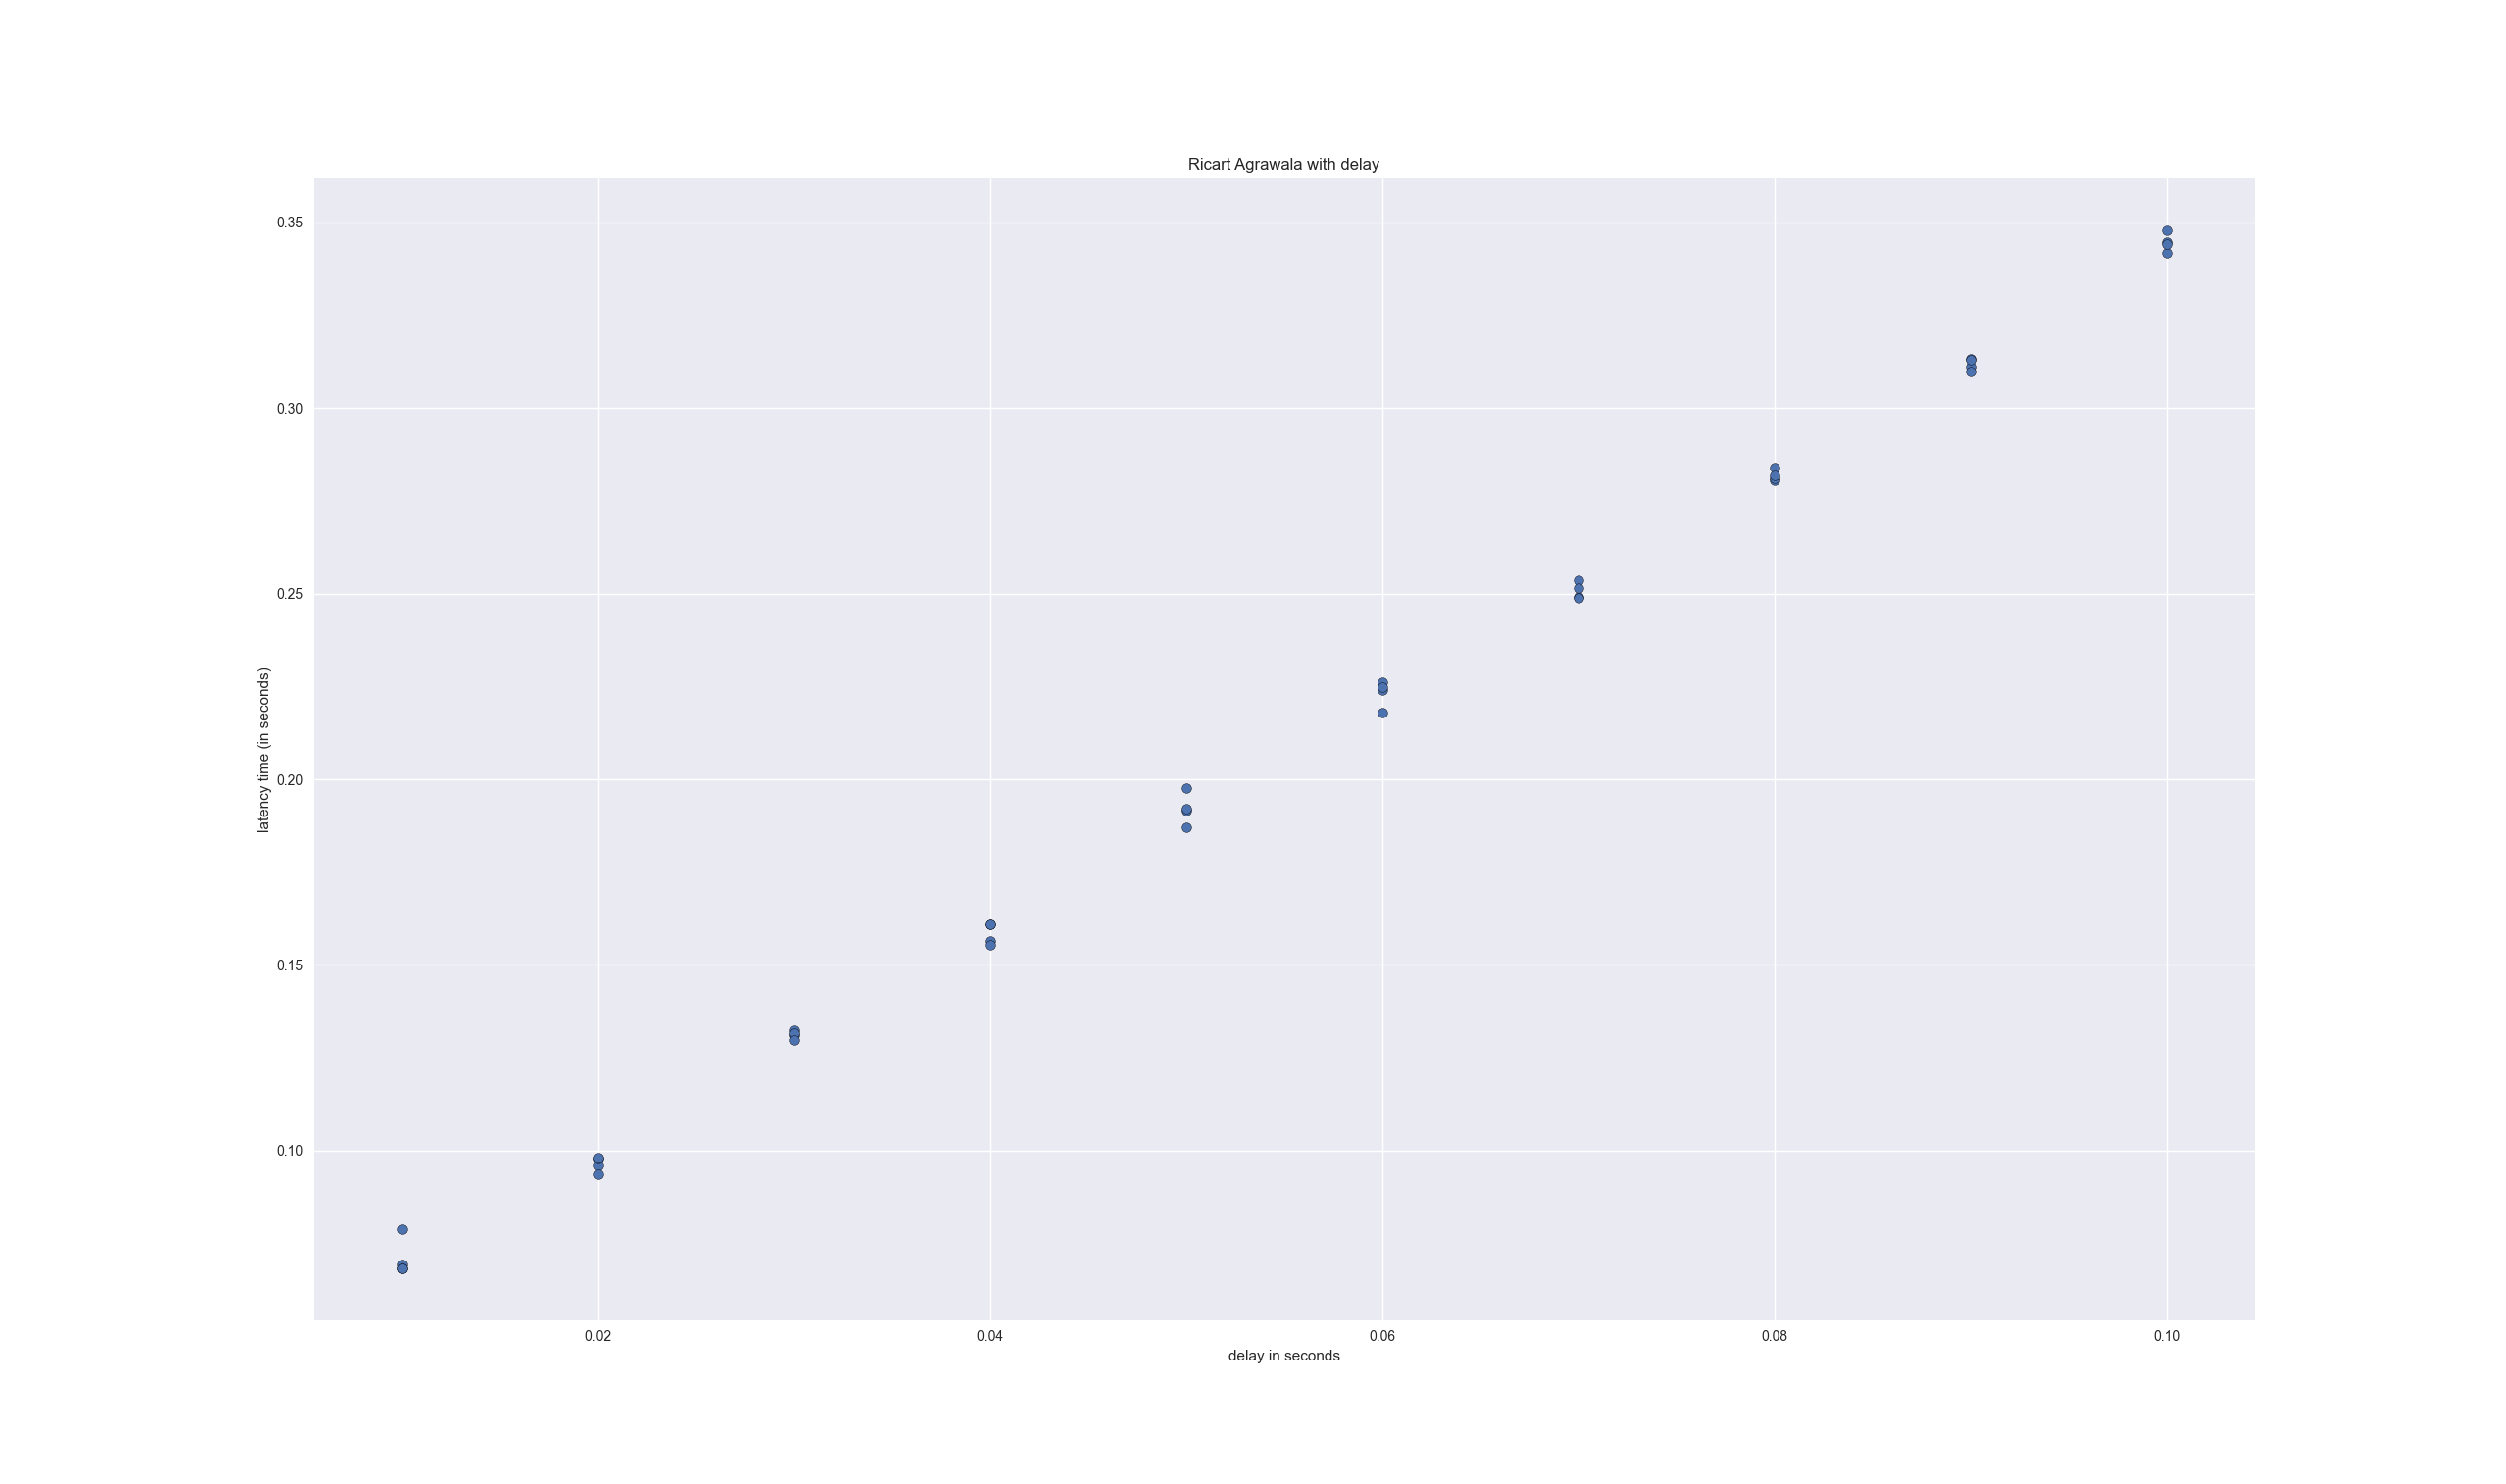
\includegraphics[width=\linewidth,height=\textheight,keepaspectratio]{ricart_agrwala_delay.png}
  \caption{Scatter plot between latency and delay in Ricart-Agrawala algorithm}
\end{figure}
